%--------------------------------------------------------------------------------------
% Este arquivo contém a introdução, objetivos e organização do trabalho
%--------------------------------------------------------------------------------------

\chapter{Introdução}

%--------------------------------------------------------------------------------------



A admiração e a curiosidade da humanidade pelo espaço vêm desde a pré-história, mas apenas através das descobertas de Isaac Newton, no Cálculo e na Física há 300 anos, a humanidade pôde trilhar um caminho, ao menos teórico rumo ao espaço. Porém, as tecnologias básicas à exploração espacial como rádio, só foram inventadas já no final do século XIX, dois séculos depois das descobertas de Newton \cite{Burgess2021}. No início do Século XX, o físico experimental Robert Goddard ansiava por provar que os foguetes poderiam ser motores no vácuo através da 3° lei de Newton (ação e reação). Conseguindo construir e lançar o primeiro foguete de propulsão líquida em 1926 visto na figura\ref{fig:Primeiro-foguete}.









\begin{figure}[ht]
    \centering
    \caption{Dr. Robert H. Goddard é mostrado em pé com o primeiro foguete de propulsão líquida do mundo em Auburn, MA, 16 de março de 1926.}
    \begin{center}
        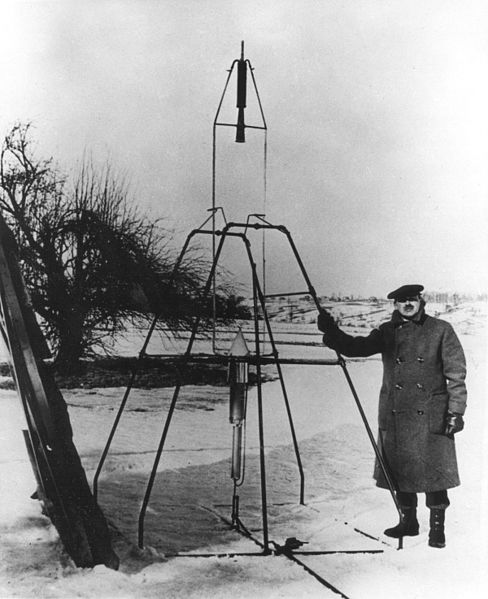
\includegraphics[width=0.35\textwidth]{img/primeirofoguete.jpg}
    \end{center}
    \vspace{-0.5cm}
    \legend{\ABNTEXfontereduzida \textbf{Fonte:} 
    \citeonline{Imagem_Primeiro_foguete}.}
   \label{fig:Primeiro-foguete}
\end{figure}.


Com o mundo entrando na Segunda Guerra Mundial, lamentavelmente a primeira aplicação dos foguetes não foi para o benefício da humanidade, sendo utilizado como meio de lançar bombas muito mais rápidas, sem os custos operacionais ou possíveis perdas de aviões e pilotos. Felizmente essa tecnologia só foi utilizada já no final da guerra, não causando tantos estragos. O míssil V2 mostrado na figura \ref{fig:foguete-V2} foi desenvolvido pelo engenheiro mecânico alemão Wernher Von Braun, Arthur Rudolph, Kurt H. Debus e outros. Logo depois da guerra, o míssil V2 foi utilizado para outras finalidades, por exemplo, responsável por tirar a 1° foto da terra a uma altitude acima da linha de Kármán \footnotemark{}  aproximadamente 104 km, em 1946.   


 




\begin{figure}[ht]
    \centering
    \caption{Míssil balístico V2 sendo preparado para lançamento em Cuxhaven, na Alemanha, 15 de  outubro de 1945.}
    \begin{center}
        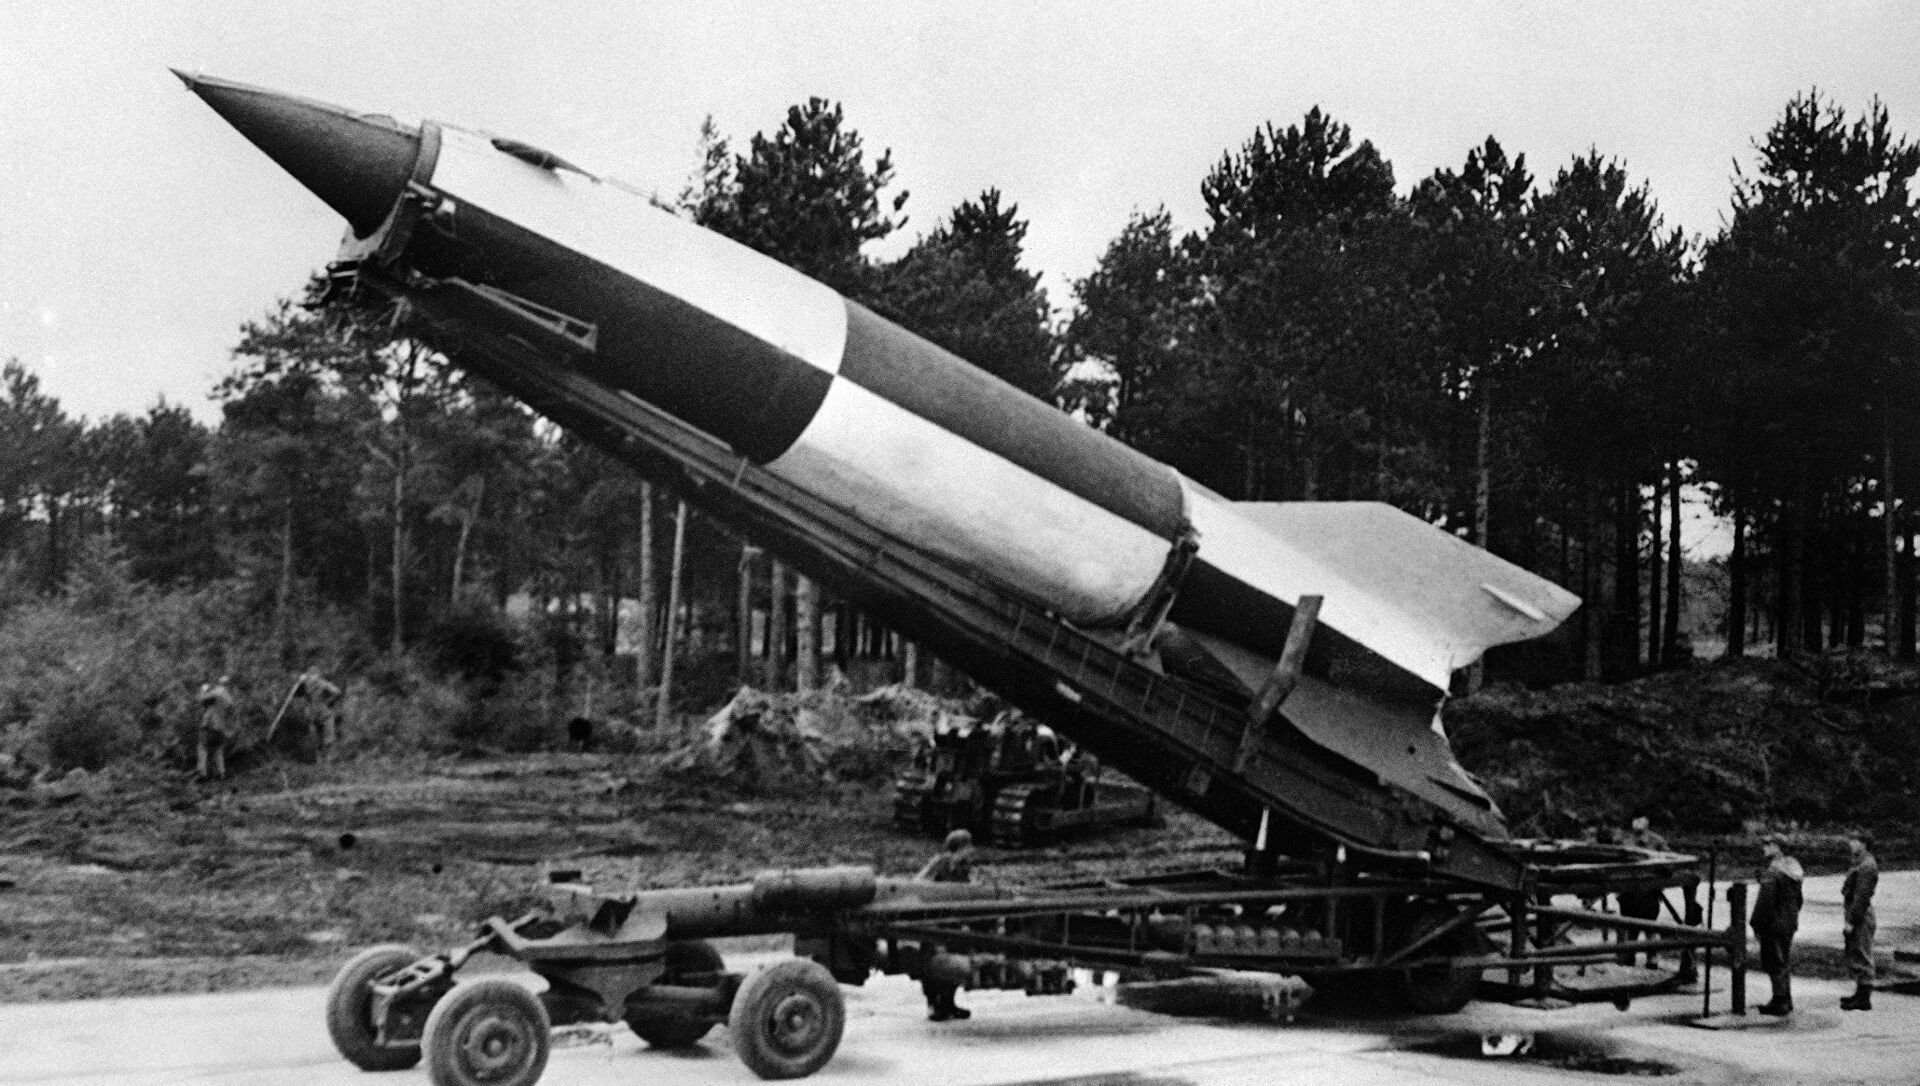
\includegraphics[width=0.5\textwidth]{img/missil_balistico_V2.jpg}
    \end{center}
    \vspace{-0.5cm}
    \legend{\ABNTEXfontereduzida \textbf{Fonte:} 
    \citeonline{Imagem_MissilV2}.}
    \label{fig:foguete-V2}
\end{figure}




.


Com o fim da Guerra, Países como os Estados Unidos (EUA) e a União Soviética (URSS) tiveram grande interesse nos cientistas e no projeto do V2, já que se tratava de uma tecnologia estratégica para o país. Tendo avanços significativos em ambos os lados como, no lado da URSS, o lançamento do primeiro satélite artificial da Terra, o Sputnik 1 em 1957, o primeiro homem e mulher a ficar na órbita da terra em 1961 e 1963, respectivamente. E pelo lado dos EUA, a chegada do homem à Lua, em 1969, através do foguete Saturno V como mostra a figura \ref{fig:Saturno-V}    \cite{UmaBreveHistoriadaConquistaEspacial}.
 

\begin{figure}[ht]
    \centering
    \caption{O foguete Saturno V preparado para o lançamento da missão Apollo 8 do Centro Espacial Kennedy em 1968.}
    \begin{center}
        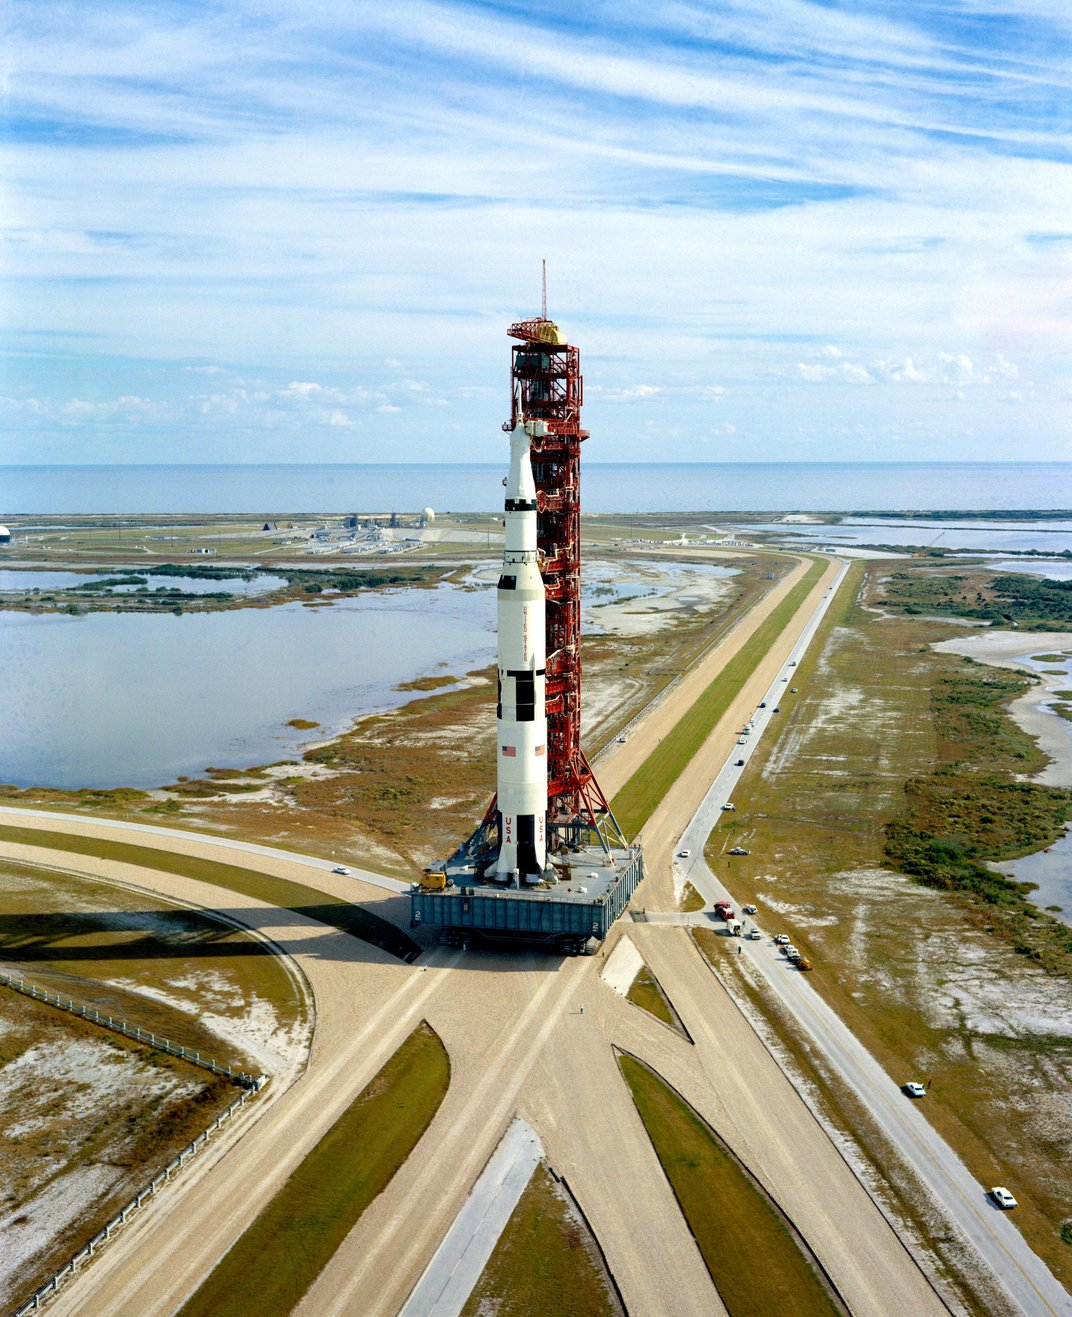
\includegraphics[width=0.35\textwidth]{img/saturn V.jpg}
    \end{center}
    \vspace{-0.5cm}
    \legend{\ABNTEXfontereduzida \textbf{Fonte:}
    \citeonline{Imagem_SaturnV}.}
    \label{fig:Saturno-V}
\end{figure}
.
 

\footnotetext{Linha de Kármán é utilizado para definir o limite entre a atmosfera terrestre e o espaço exterior que fica a uma altitude de 100 km acima do nível do mar.}





Já no Brasil, o Departamento de Ciência e Tecnologia Aeroespacial (DCTA) foi fundado em 1946, depois os principais institutos como o Centro Técnico Aeroespacial (CTA) e o Instituto Tecnológico de Aeronáutica (ITA) em 1950. Esses centros e institutos foram criados visando obter a autossuficiência do Brasil na formação de profissionais qualificados para trabalhar na área da aeronáutica e aeroespacial. Porém, só na década de 1960, o Brasil deu início ao desenvolvimento dos primeiros foguetes. Como os de sondagem que tem o propósito de levar pequenas cargas úteis para a alta atmosfera, realizando pesquisas e experiências \cite{INTRODUCAO_TECNOLOGIA_FOGUETES}.


O primeiro foi o Sonda I feito em 1967, o segundo o Sonda II em 1970 chegando a um apogeu  \footnotemark{} de 96 km, depois o  sonda III em 1976, com apogeu de 700 km. Até que em 1984 o auge da família com o sonda IV chegando a um apogeu de 700 km e conseguindo carregar até 500 kg de carga útil foi a base para a construção do Veículo lançador de satélites (VLS) \cite{Foguetes-AEB}.


Devido ao baixíssimo orçamento pelo governo e as grandes dificuldades na importação de componentes estratégicos devido aos embargos dos EUA, o programa do VLS só conseguiu realizar 3 tentativas com a última ocasionando a destruição da base e na morte de 21 pessoas em 2003. Ressurgindo apenas em 2010 o interesse em lançamentos de micro e nanossatélites e apenas em 2014 o Brasil em parceria com a Alemanha, deu início ao desenvolvendo do veículo de sondagem VS 50 que será base para a construção do veículo lançador de microssatélites (VLM-1). Com o novo projeto do VLM-1 o antigo VLS teve seu cancelamento definitivo em 2016 \cite{INTRODUCAO_TECNOLOGIA_FOGUETES}.



Visando possibilitar que estudantes possam participar de atividades voltadas ao desenvolvimento aeroespacial, a COBRUF Association é uma iniciativa privada New Space criada em 2012 por 10 estudantes de graduação da UFABC e que tem uma forte influência na coordenação de diversas operações experimentais de lançamento de foguetes com a Força Aérea Brasileira. Além disso, ela é responsável por promover diversas competições de foguetemodelismo nacional e internacional, impulsionando assim, o conhecimento técnico de diversos estudantes brasileiros nessa área tão escassa de profissionais\cite{Cobruf}.


Com o intuito de que a Universidade Federal do Vale do São Francisco -(UNIVASF) também entrasse nessa competição de foguetemodelismo, a equipe Cactus Rockets Design foi criada em 2019, por estudantes e professores. Visando contribuir com a equipe para que ela consiga alcançar o seu objetivo de construir foguetes modelos intermediários e avançados, esse trabalho de conclusão de curso foi desenvolvido para ajudar na coleta de dados dos sensores e na telemetria dos foguetes modelos projetados pela Cactus Rockets.



 \footnotetext{Apogeu na engenharia aeroespacial é a altura máxima em que o foguete pode atingir em relação a terra depois que todo o seu combustível é queimado.}

\newpage

\section{Justificativa}

A competição de foguetes organizada pela COBRUF dá a possibilidade para que estudantes de engenharia possam entrar em contato com o ambiente da engenharia aeroespacial, onde as necessidades e as exigências aos sistemas embarcados estão cada vez mais altas. Com o intuito de contribuir com a equipe Cactus Rockts em seu objetivo de construir foguetes intermediários e avançados, propomos um sistema embarcado para o foguete e um sistema externo no solo para receber os dados via telemetria. Através do sistema será possível obter os dados necessários para validar os cálculos e simulações feitas pela equipe e assim facilitar a identificação de erros de projeto e consequentemente favorecer melhorias futuras no desempenho dos foguetes projetados pela equipe Cactus Rockts.


\section{Objetivos gerais}

Possibilitar que a equipe de foguetemodelismo chamada Cactus Rockets Design da Universidade Federal do Vale do São Francisco possa obter os dados relevantes sobre os foguetes projetados. E assim, ser capaz de verificar se seus cálculos e simulações estão de acordo com a realidade mensurada de seus protótipos.



\section{Objetivos específicos}


\begin{itemize}
	\item Definir quais parâmetros são necessários e os sensores para mensurar tais parâmetros;
	
    \item Definir qual o microcontrolador será utilizado com base em um custo-benefício;
    
    \item Definir qual rádio apresenta um melhor custo-benefício para o projeto;
    
    \item Teste em bancada dos sensores;
    
    \item Teste em bancada do rádio;
    
    \item Teste do rádio em campo aberto para obter uma estimativa do alcance;
    
    \item Desenvolver o protótipo.
\end{itemize}





\section{Organização do trabalho}


O presente trabalho foi dividido em 3 etapas. A primeira etapa, trata-se de um resumo da história do foguete no mundo e no Brasil e a motivação para o desenvolvimento deste projeto. Na segunda, etapa é desenvolvida a fundamentação teórica que servirá como base para a realização deste trabalho. Por fim, a terceira etapa relata a metodologia utilizada neste projeto. Tendo no final da terceira etapa, um cronograma de atividades a serem executadas no Trabalho de conclusão II (TCC II).




